%
% spanningtree.tex
%
% (c) 2019 Prof Dr Andreas Müller, Hochschule Rapperswil
%
\begin{frame}
\frametitle{Spannbäume}

\vspace{-16pt}

\begin{columns}[t]

\begin{column}{0.40\hsize}
\begin{block}{Netzwerk}
Alle Knoten erreichen, Schleifen vermeiden $\Rightarrow$ Spannbaum
\vspace{-15pt}
\begin{center}
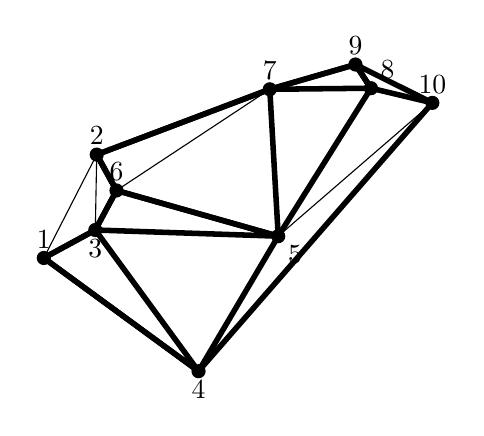
\begin{tikzpicture}[>=latex,scale=0.18]

\coordinate (A) at ( 1.2927,-15.0076);
\coordinate (B) at ( 5.0261,- 7.7143);
\coordinate (C) at ( 4.9260,-13.0335);
\coordinate (D) at (12.2094,-22.9960);
\coordinate (F) at (17.8334,-13.4687);
\coordinate (G) at ( 6.4208,-10.2438);
\coordinate (H) at (17.2367,- 3.1047);
\coordinate (K) at (24.3760,- 3.0293);
\coordinate (L) at (23.2834,- 1.3563);
\coordinate (M) at (28.7093,- 4.0627);

\fill (A) circle[radius=0.5];
\fill (B) circle[radius=0.5];
\fill (C) circle[radius=0.5];
\fill (D) circle[radius=0.5];
\fill (F) circle[radius=0.5];
\fill (G) circle[radius=0.5];
\fill (H) circle[radius=0.5];
\fill (K) circle[radius=0.5];
\fill (L) circle[radius=0.5];
\fill (M) circle[radius=0.5];

%\uncover<1-4>{
%\node at (A) [above] {$A$};
%\node at (B) [above] {$B$};
%\node at (C) [below] {$C$};
%\node at (D) [below] {$D$};
%\node at (F) [below right] {$F$};
%\node at (G) [above] {$G$};
%\node at (H) [above] {$H$};
%\node at (K) [above right] {$K$};
%\node at (L) [above] {$L$};
%\node at (M) [above] {$M$};
%}

\uncover<5->{
\node at (A) [above] {$1$};
\node at (B) [above] {$2$};
\node at (C) [below] {$3$};
\node at (D) [below] {$4$};
\node at (F) [below right] {$5$};
\node at (G) [above] {$6$};
\node at (H) [above] {$7$};
\node at (K) [above right] {$8$};
\node at (L) [above] {$9$};
\node at (M) [above] {$10$};
}

\draw (L)--(H);
\draw (L)--(K);
\draw (L)--(M);

\draw (H)--(B);
\draw (H)--(G);
\draw (H)--(F);
\draw (H)--(K);

\draw (K)--(F);
\draw (K)--(M);

\draw (M)--(F);
\draw (M)--(D);

\draw (B)--(A);
\draw (B)--(C);
\draw (B)--(G);

\draw (G)--(C);
\draw (G)--(F);

\draw (F)--(D);

\draw (C)--(F);
\draw (C)--(A);
\draw (C)--(D);

\draw (A)--(D);

\uncover<2>{
\draw[line width=2pt,join=round]
	(A)--(D)--(C)--(F)--(G)--(B)--(H)--(K)--(L)--(M);
}

\uncover<3>{
\draw[line width=2pt,join=round]
	(M)--(D)--(A)--(C)--(G)--(B)--(H)--(L)--(K)--(F);
}

\uncover<4->{
\draw[line width=2pt] (M)--(K)--(L)--(H)--(F)--(D);
\draw[line width=2pt] (F)--(G)--(C)--(A);
\draw[line width=2pt] (G)--(B);
}

\end{tikzpicture}
\end{center}
\vspace{-10pt}
Wieviele Spannbäume gibt es?
\end{block}
\end{column}

\begin{column}{0.56\hsize}
\uncover<5->{%
\begin{block}{Laplace-Matrix}
\vspace{-15pt}
\[
L=
\tiny
\begin{pmatrix}
 3&-1&-1&-1& 0& 0& 0& 0& 0& 0\\
-1& 4&-1& 0& 0&-1&-1& 0& 0& 0\\
-1&-1& 5&-1&-1&-1& 0& 0& 0& 0\\
-1& 0&-1& 4&-1& 0& 0& 0& 0&-1\\
 0& 0&-1&-1& 6&-1&-1&-1& 0&-1\\
 0&-1&-1& 0&-1& 4&-1& 0& 0& 0\\
 0&-1& 0& 0&-1&-1& 5&-1&-1& 0\\
 0& 0& 0& 0&-1& 0&-1& 4&-1&-1\\
 0& 0& 0& 0& 0& 0&-1&-1& 3&-1\\
 0& 0& 0&-1&-1& 0& 0&-1&-1& 4\\
\end{pmatrix}
\]
\end{block}}
\vspace{-15pt}
\uncover<6->{%
\begin{block}{Satz von Kirchhoff}
Die Anzahl der Spannbäume eines Netzwerkes ist ein Kofaktor
des Laplaceoperators
\vspace{-5pt}
\[
\det L_{ij} = 
\left|
L\text{ ohne }\left\{\begin{array}{c}\text{Zeile $i$}\\\text{Spalte $j$}\end{array}\right.
\right|
\]
\end{block}}
\vspace{-12pt}
\uncover<7->{%
{\usebeamercolor[fg]{title}Beispiel:} 41524
}

\end{column}

\end{columns}

\end{frame}
